%% FILTRES %%

\section{Filtres}
	\begin{frame}{Filtres}
		\begin{overprint}
		\begin{enumerate}
			\only<1>{
				\item[]
					\begin{itemize}
						\item S'appliquent sur un calque, un groupe de calques ou un masque
						\item Gestion
							\begin{itemize}
							\item du flou
							\item des couleurs
							\item "d'amélioration"
							\item "artistique"
							\item etc
							\end{itemize}
						\item "Destructifs" et non modifiables par la suite $\rightarrow$ devrait changer avec GIMP 3.2
					\end{itemize}
			}

			\only<2>{
				\item[]
					\framesubtitle{Mais, à quoi ça sert Jamy?}
						\begin{itemize}
							\item Automatiser une tâche fastidieuse (filtre film, fractales, par ex.)
							\item Appliquer des effets à un calque (distorsions, transformations en peintures, par ex.)
							\item Appliquer des corrections à un calque (pixellisation ou flou gaussien, par ex.)
						\end{itemize}
			}

			\only<3>{
				\item[]
					\framesubtitle{Et donc, Jamy, comment on applique un filtre?}
						Et bien c'est très simple! Il suffit de:
						\begin{enumerate}[I]
							\item Dupliquer le calque sur lequel on va travailler
							\item Masquer le nouveau calque afin que seule la zone qu'on souhaite modifier soit touchée par le filtre
							\item Accéder aux filtres par le menu ou un clic droit
							\item Jouer avec les réglages du filtre et l'appliquer sur le calque
						\end{enumerate}

						Conseil: si on se rend compte qu'on n'a pas appliqué les bonnes options au filtre; il n'est pas nécessaire de tout recommencer depuis le début. Il suffit d'annuler ce qu'on vient de faire (Ctrl+Z ou "Edition $\rightarrow$ Annuler") et de réafficher le dernier (Maj+Ctrl+F ou "Filtres $\rightarrow$ Réafficher le dernier").
			}
		\end{enumerate}
		\end{overprint}
	\end{frame}

\begin{frame}{Filtres}
		On peut par exemple appliquer un filtre de flou gaussien à un masque, pour rendre son intégration à un montage plus discrète:
		\begin{figure}[H]
			\centering
			\begin{minipage}{.5\textwidth}
				\centering
				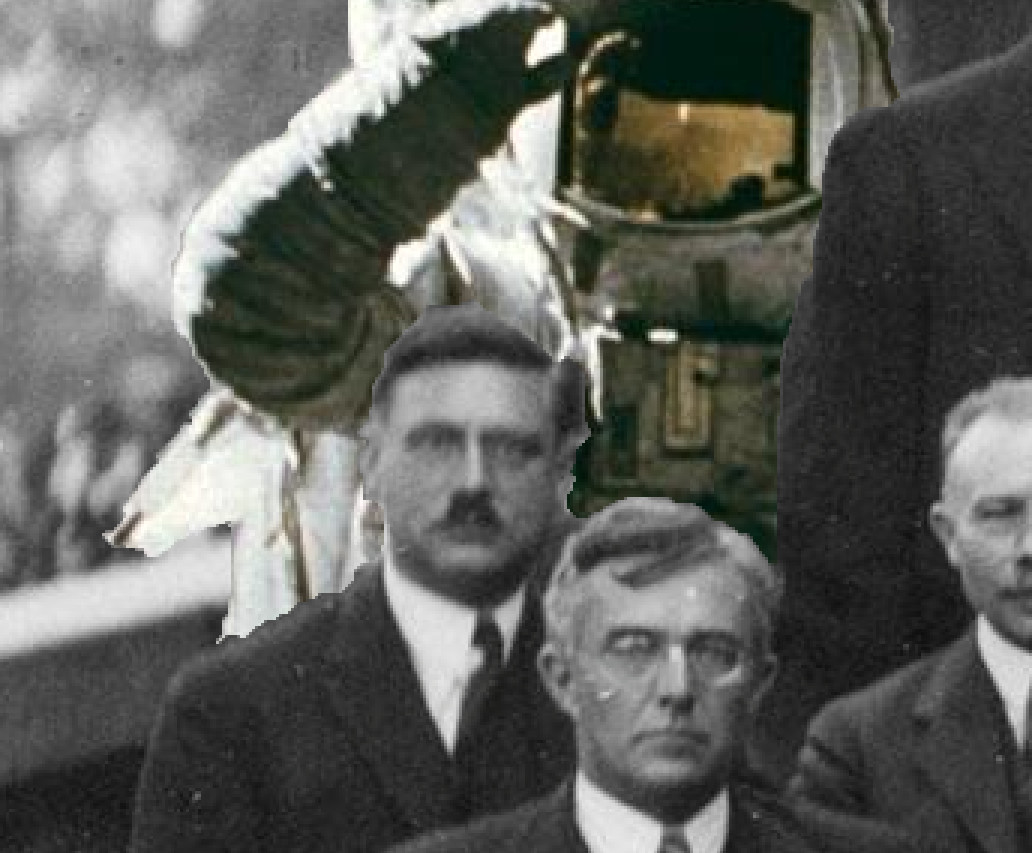
\includegraphics[height=120px]{Images/filters/astro0}
				\caption{Sans filtre appliqué}
			\end{minipage}%
			\begin{minipage}{.5\textwidth}
				\centering
				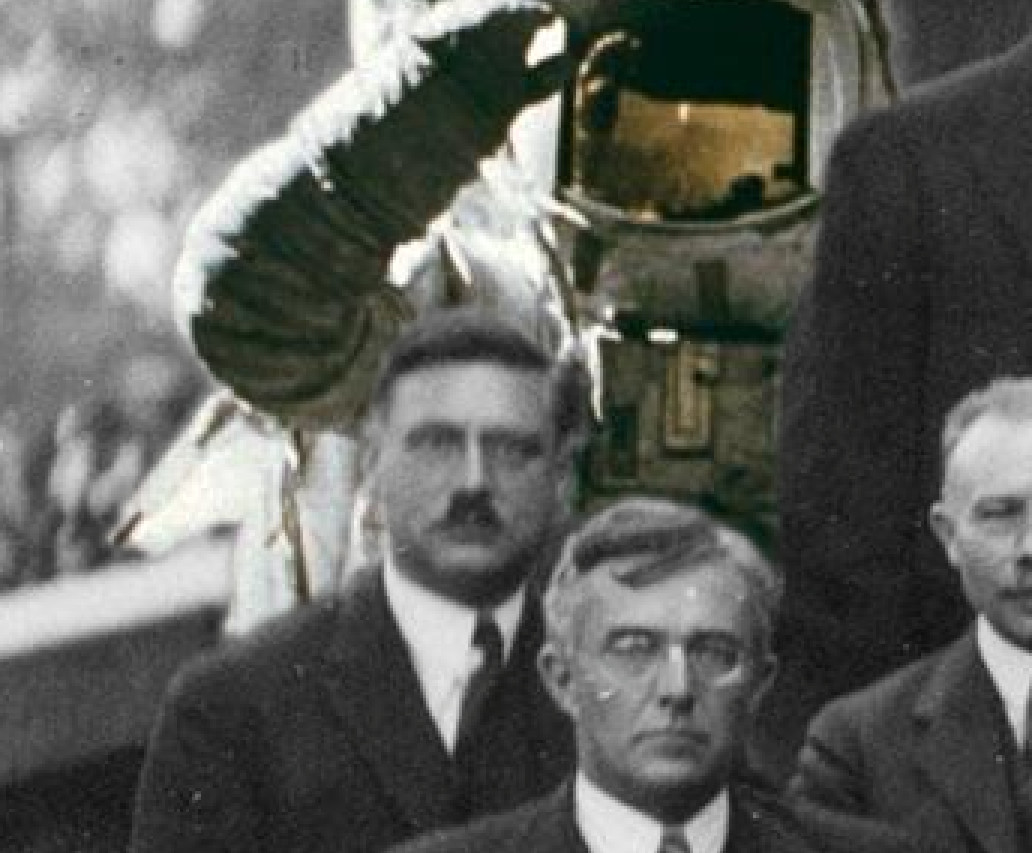
\includegraphics[height=120px]{Images/filters/astro1}
				\caption{Après application du filtre}
			\end{minipage}
		\end{figure}
\end{frame}


	\begin{frame}{Filtres}
		\begin{figure}[H]
			\centering
			\begin{minipage}{.6\textwidth}
				\centering
				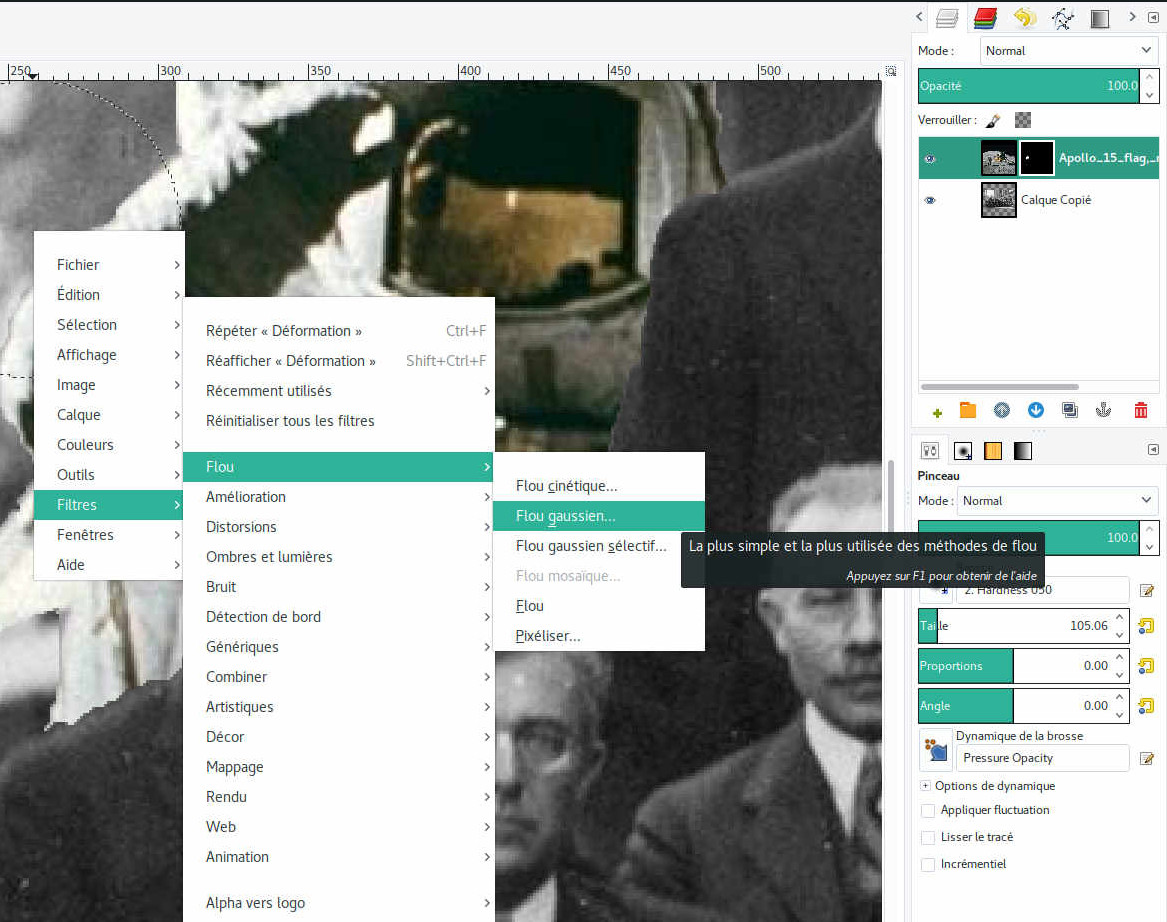
\includegraphics[height=120px]{Images/filters/astroBlur}
				\end{minipage}$\rightarrow$%
			\begin{minipage}{.4\textwidth}
				\centering
				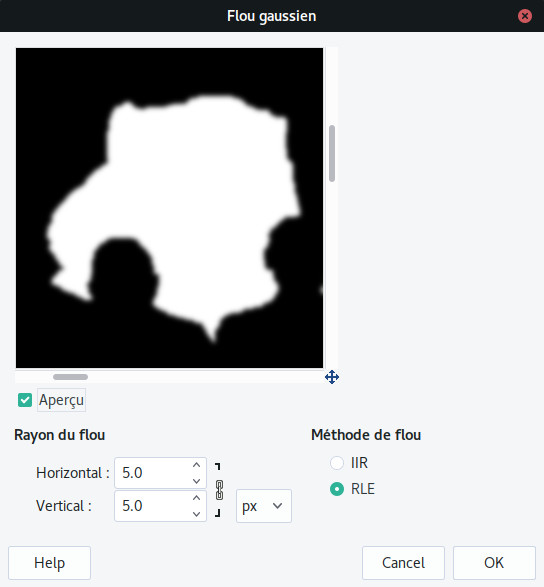
\includegraphics[height=100px]{Images/filters/gaussBlur}
				\end{minipage}

Filtres $\rightarrow$ Flou $\rightarrow$ Flou gaussien
			\end{figure}
	\end{frame}


\begin{frame}{Filtres}

	Il existe une foule d'autres filtres, certains aux effets relativement discrets ou plus "spectaculaires":

	\begin{overprint}
	\begin{enumerate}
		\only<1>{
			\item[]
				\begin{figure}[H]
					\centering
						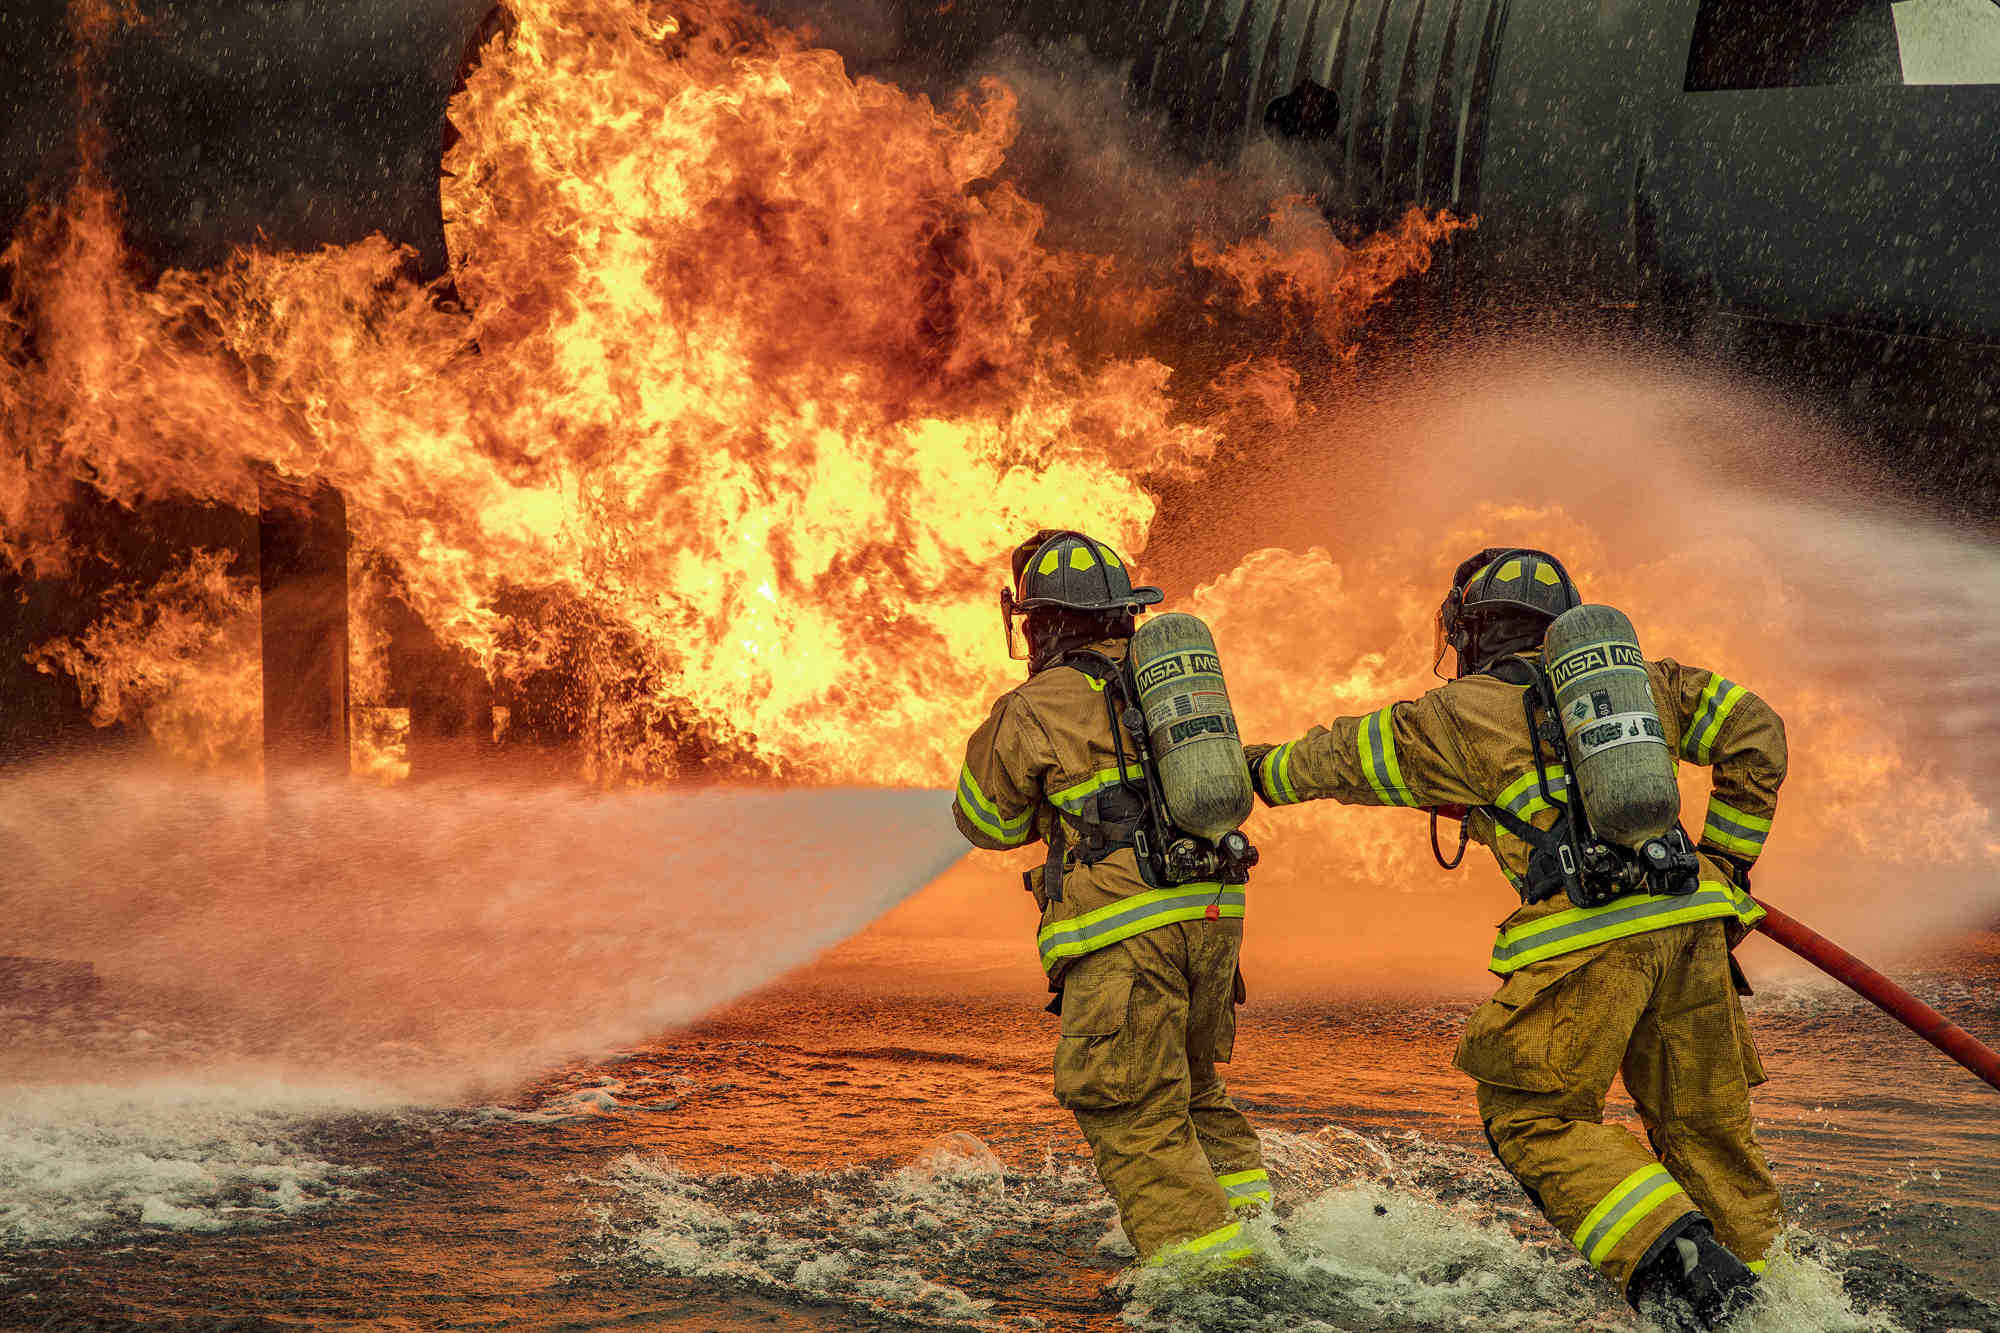
\includegraphics[height=150px]{Images/filters/compressed_original}
						\caption{\#NoFilter}
				\end{figure}
		}

		\only<2>{
			\item[]
				\begin{figure}[H]
					\centering
						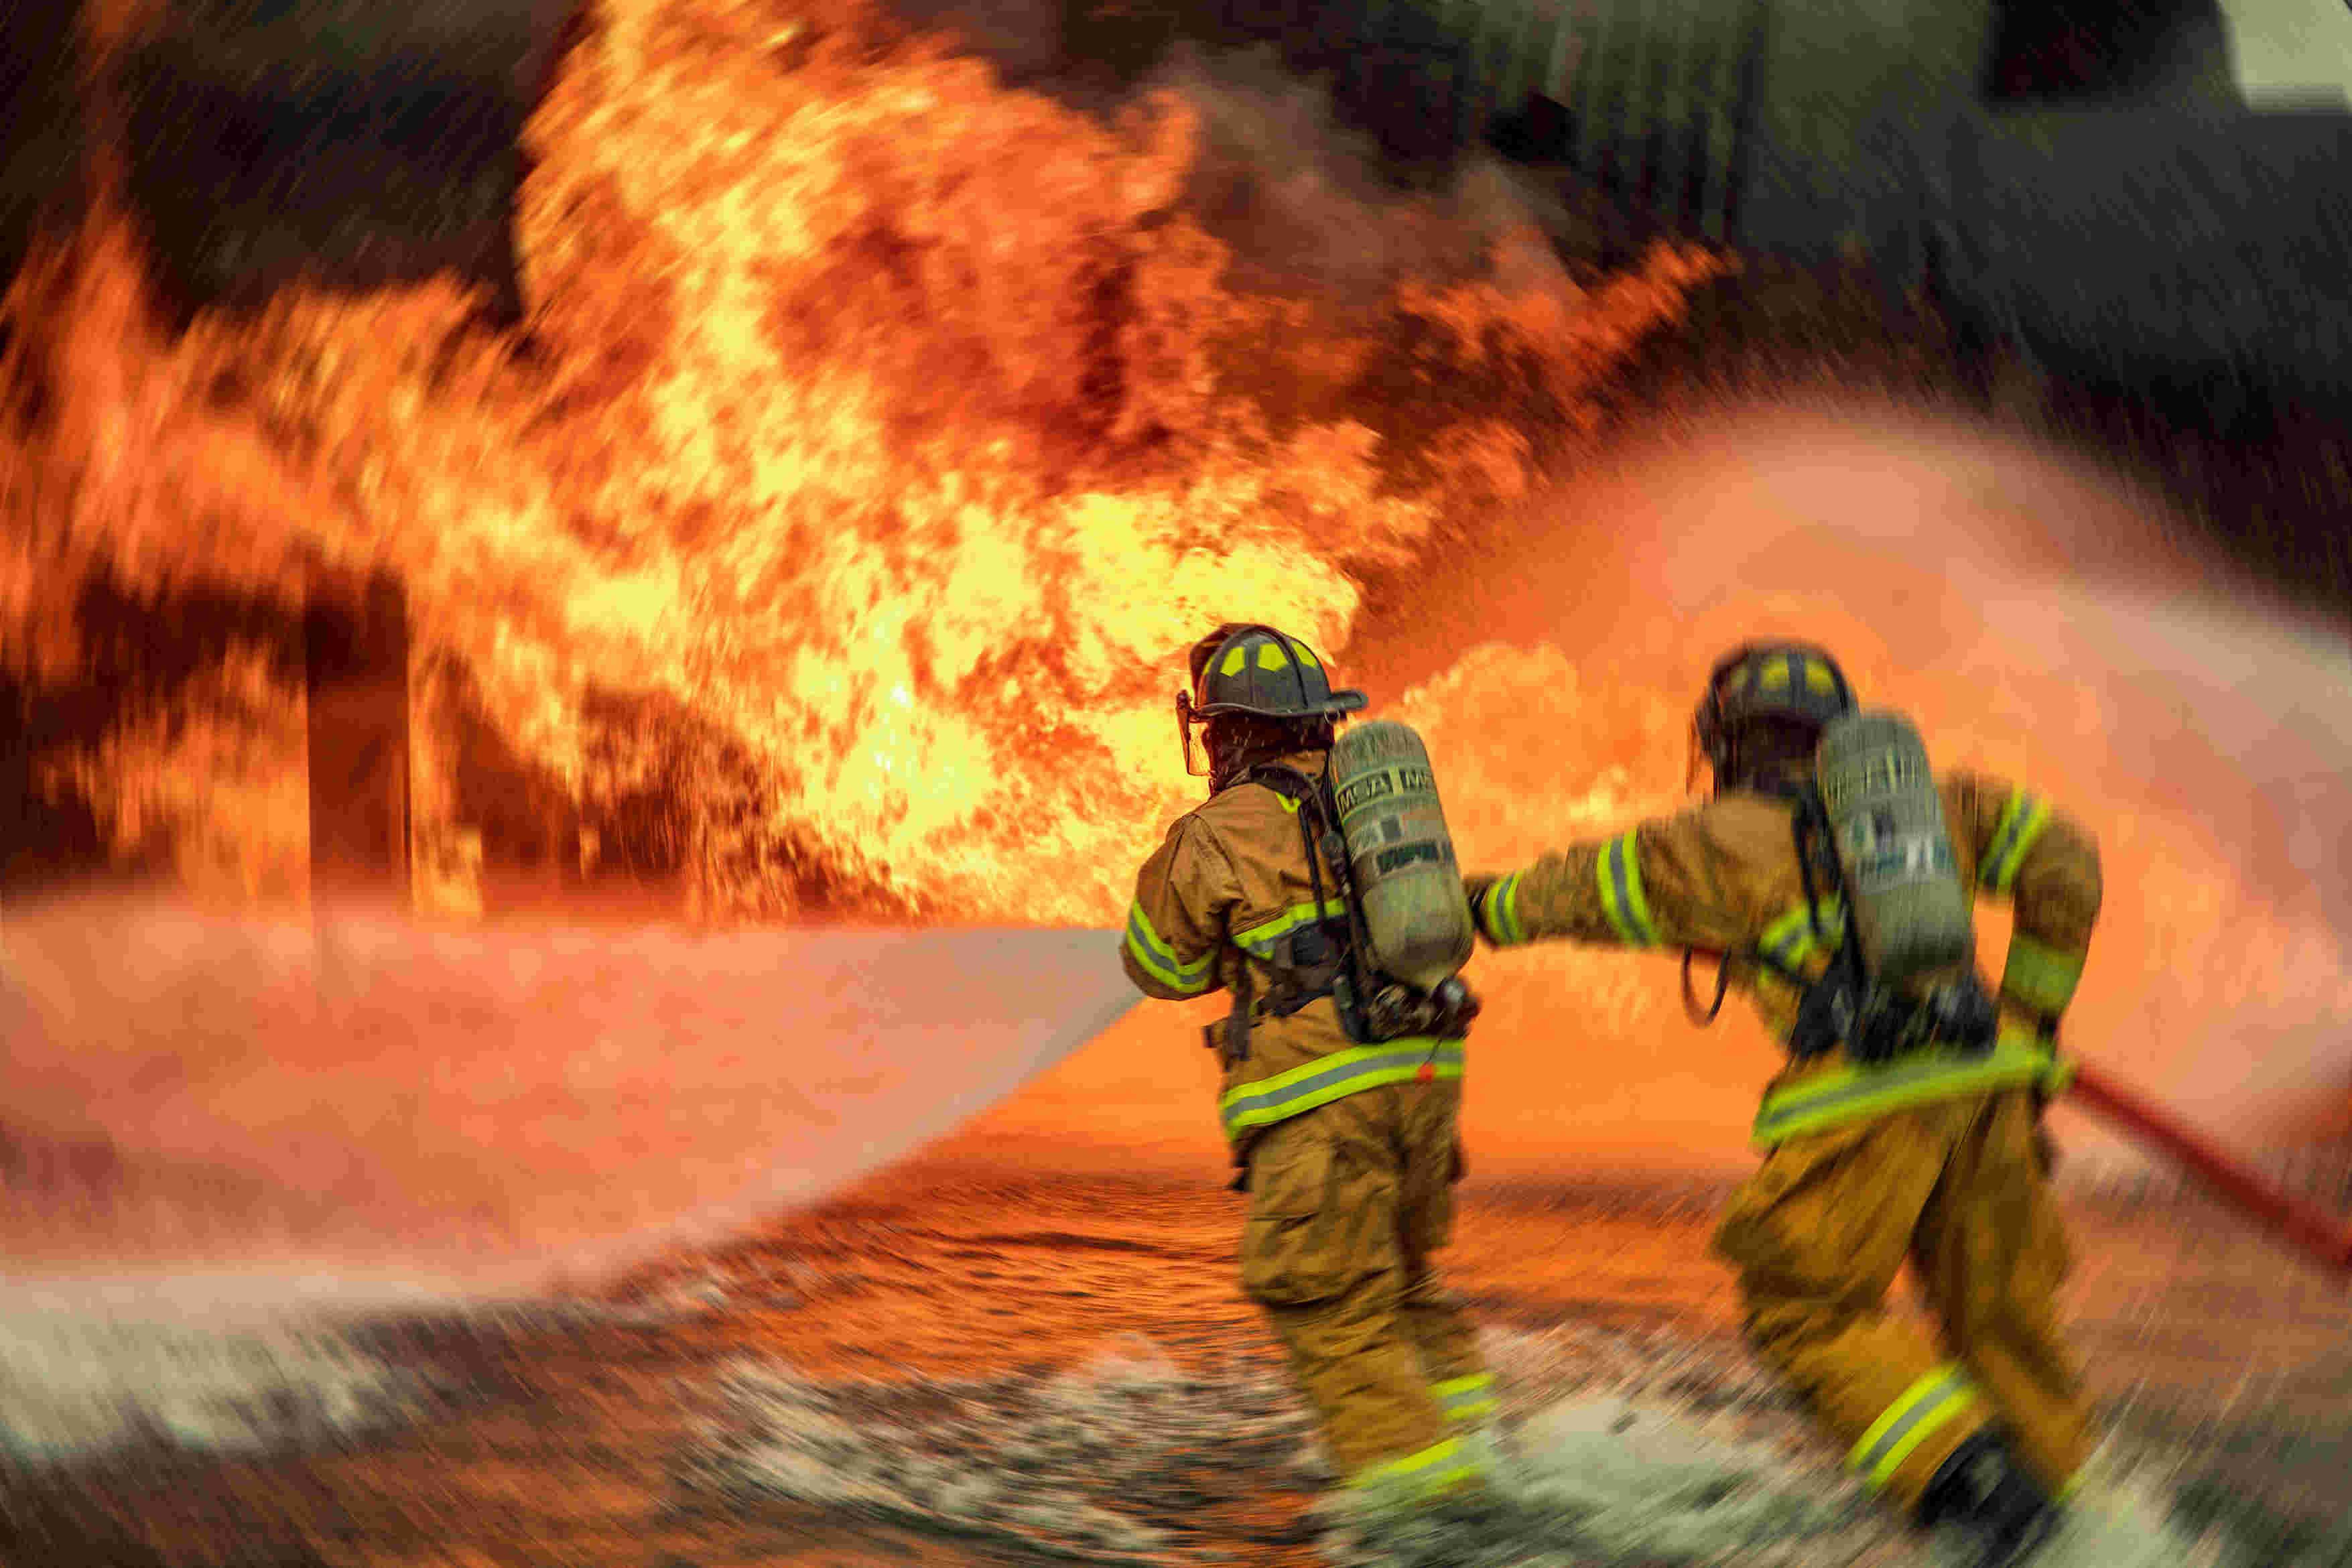
\includegraphics[height=150px]{Images/filters/motion_blur}
						\caption{Flou cinétique}
				\end{figure}
		}

		\only<3>{
			\item[]
				\begin{figure}[H]
					\centering
						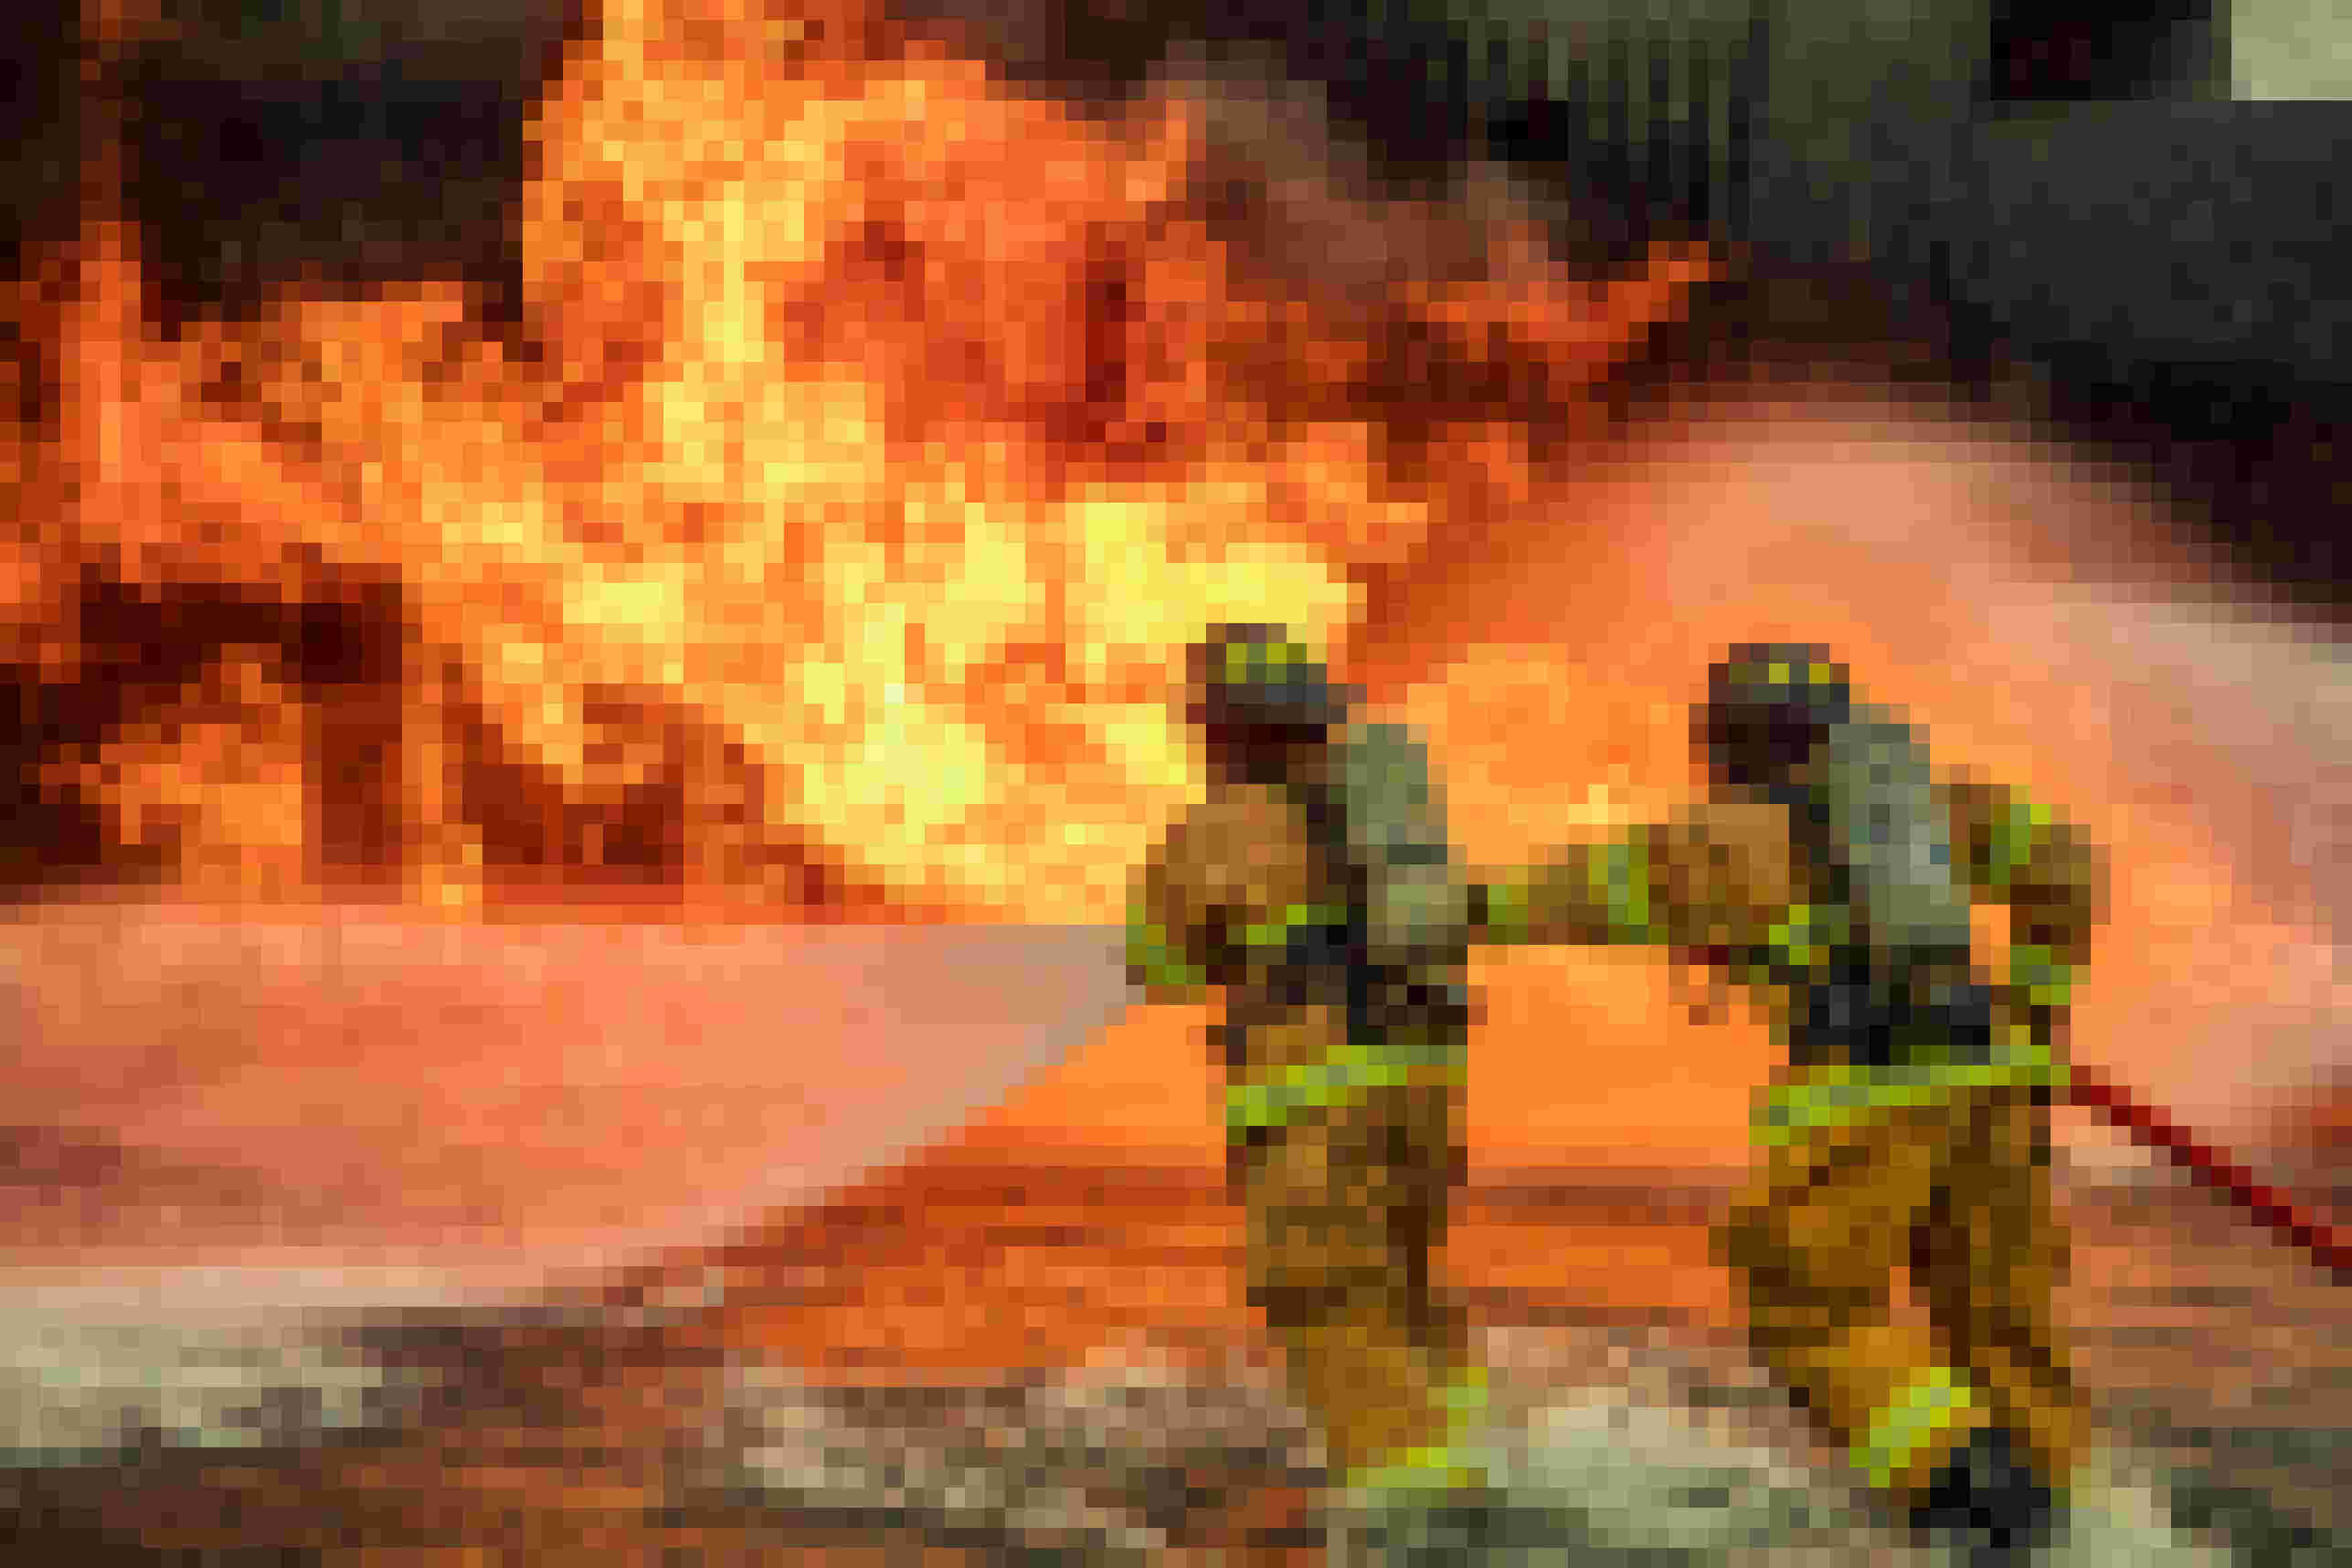
\includegraphics[height=150px]{Images/filters/pixelize}
						\caption{Pixélisé}
				\end{figure}
		}

		\only<4>{
			\item[]
				\begin{figure}[H]
					\centering
						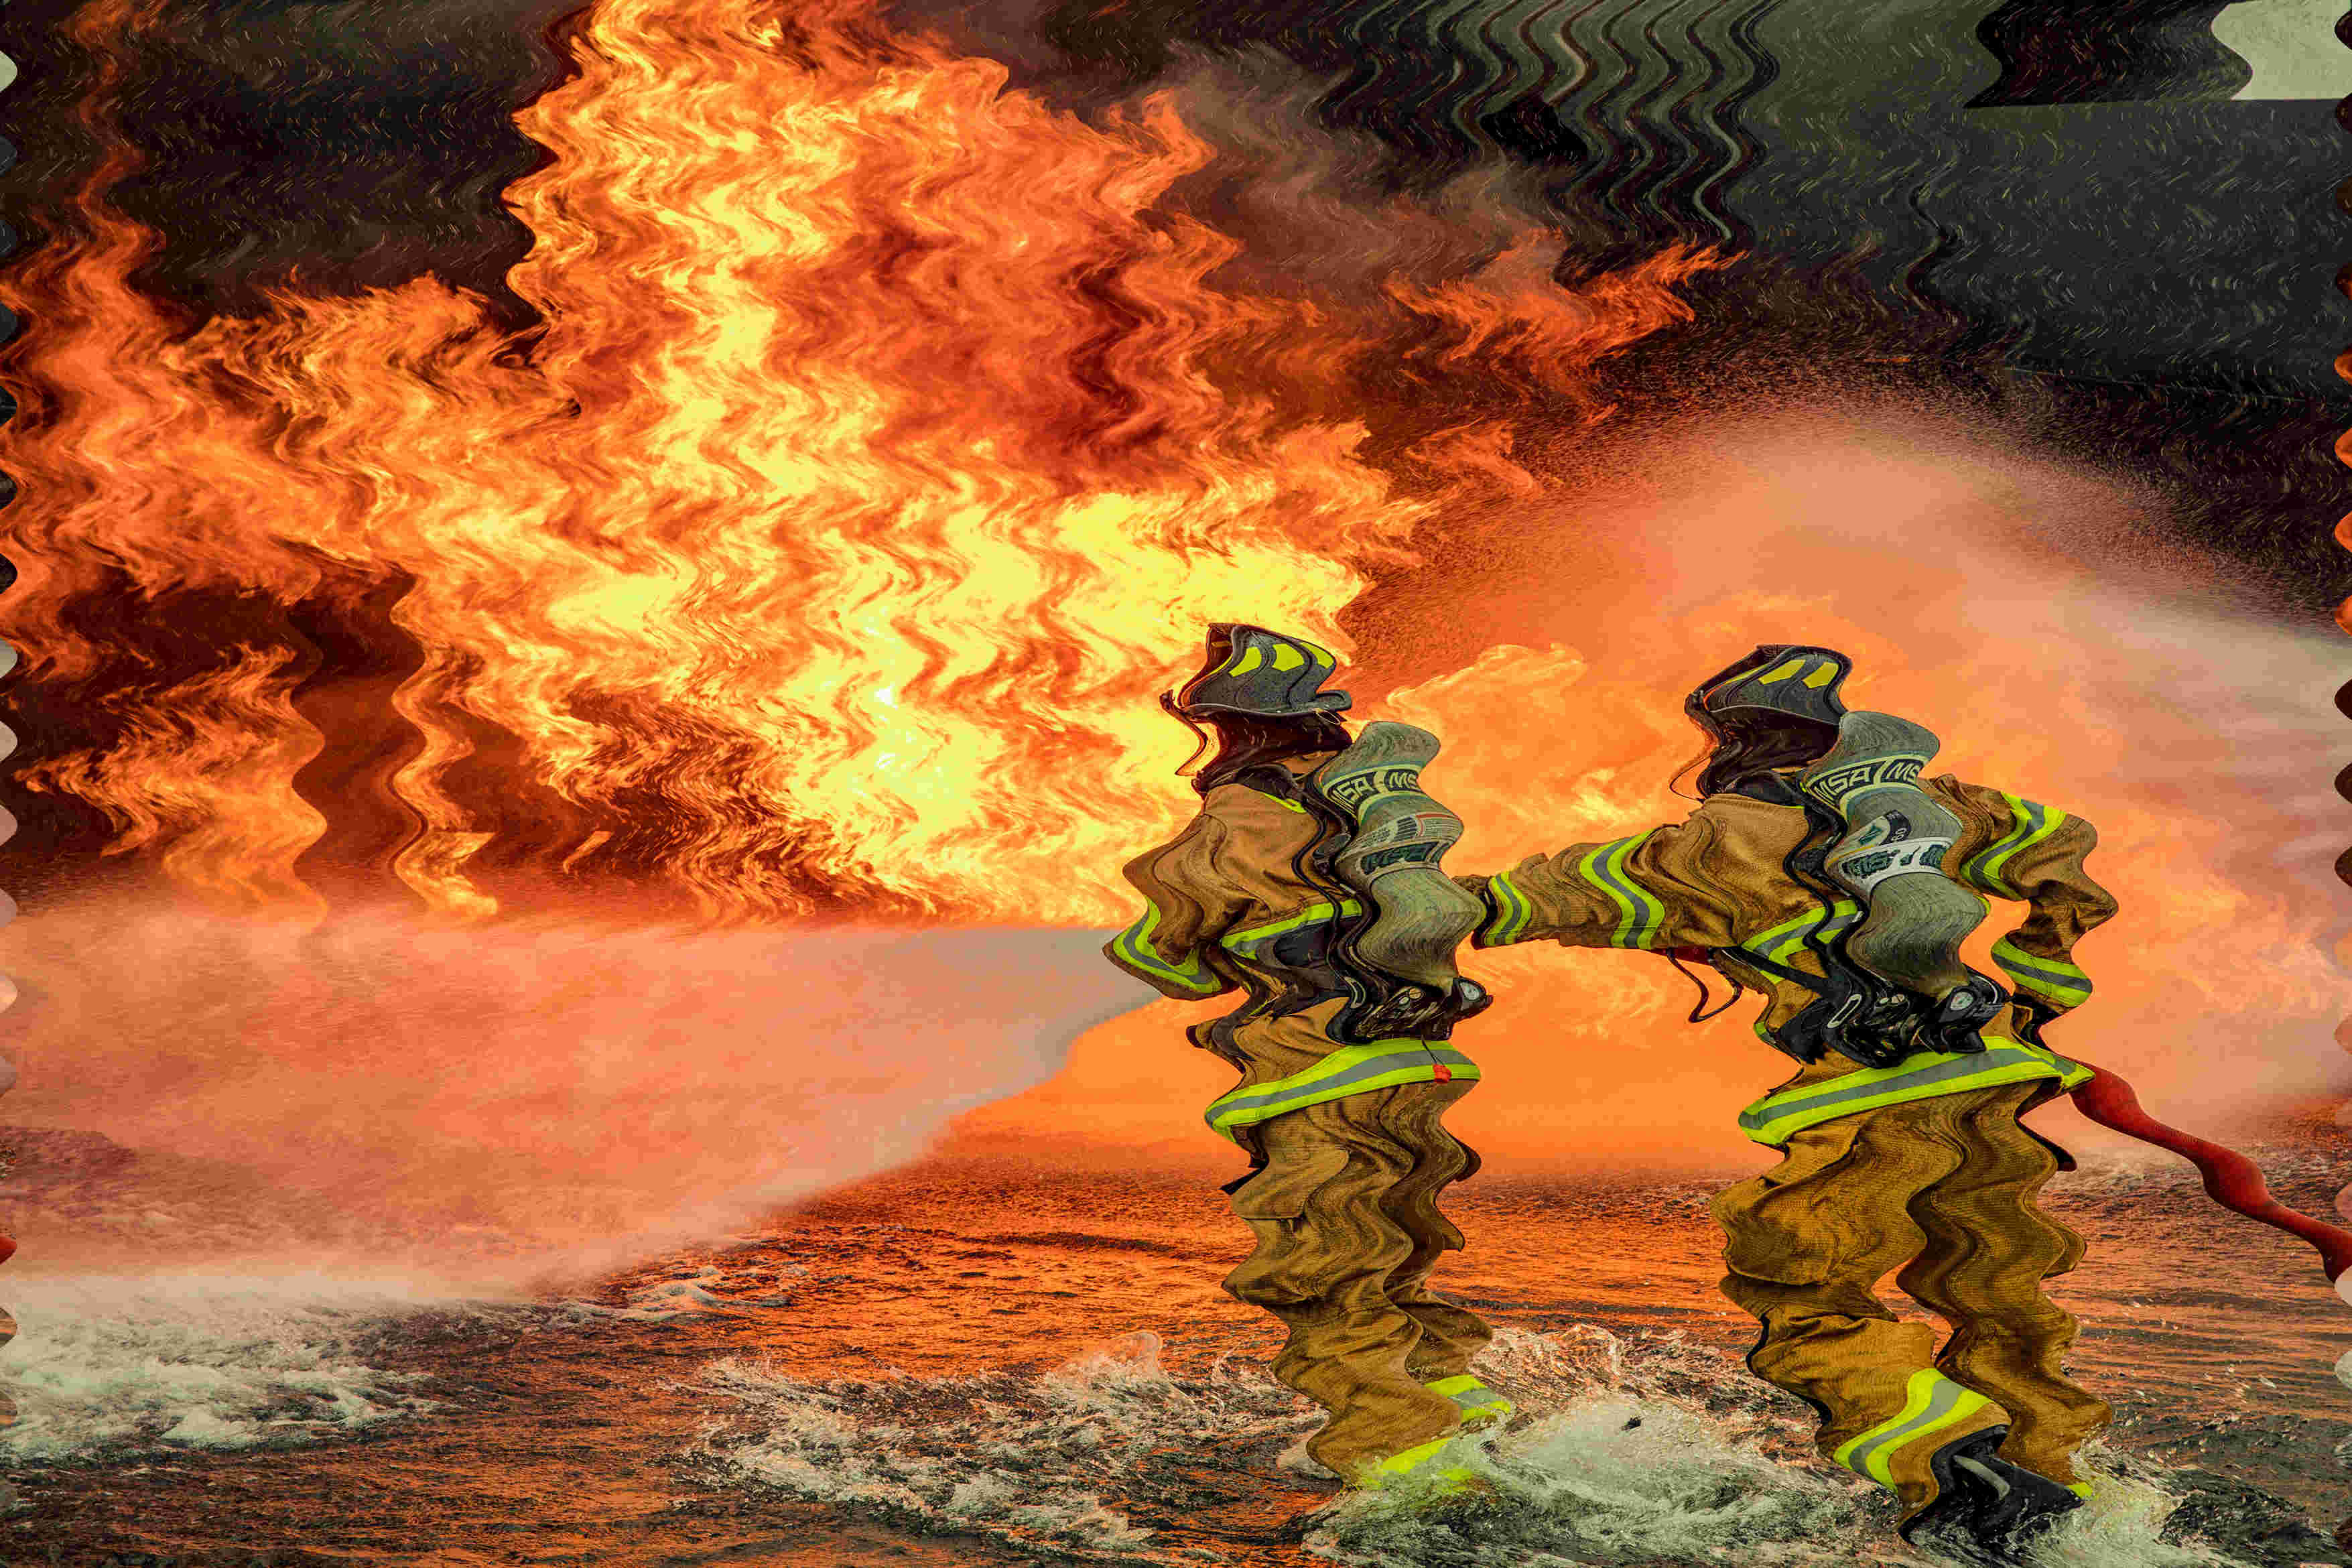
\includegraphics[height=150px]{Images/filters/ripples}
						\caption{Vagues}
				\end{figure}
		}

		\only<5>{
			\item[]
				\begin{figure}[H]
					\centering
						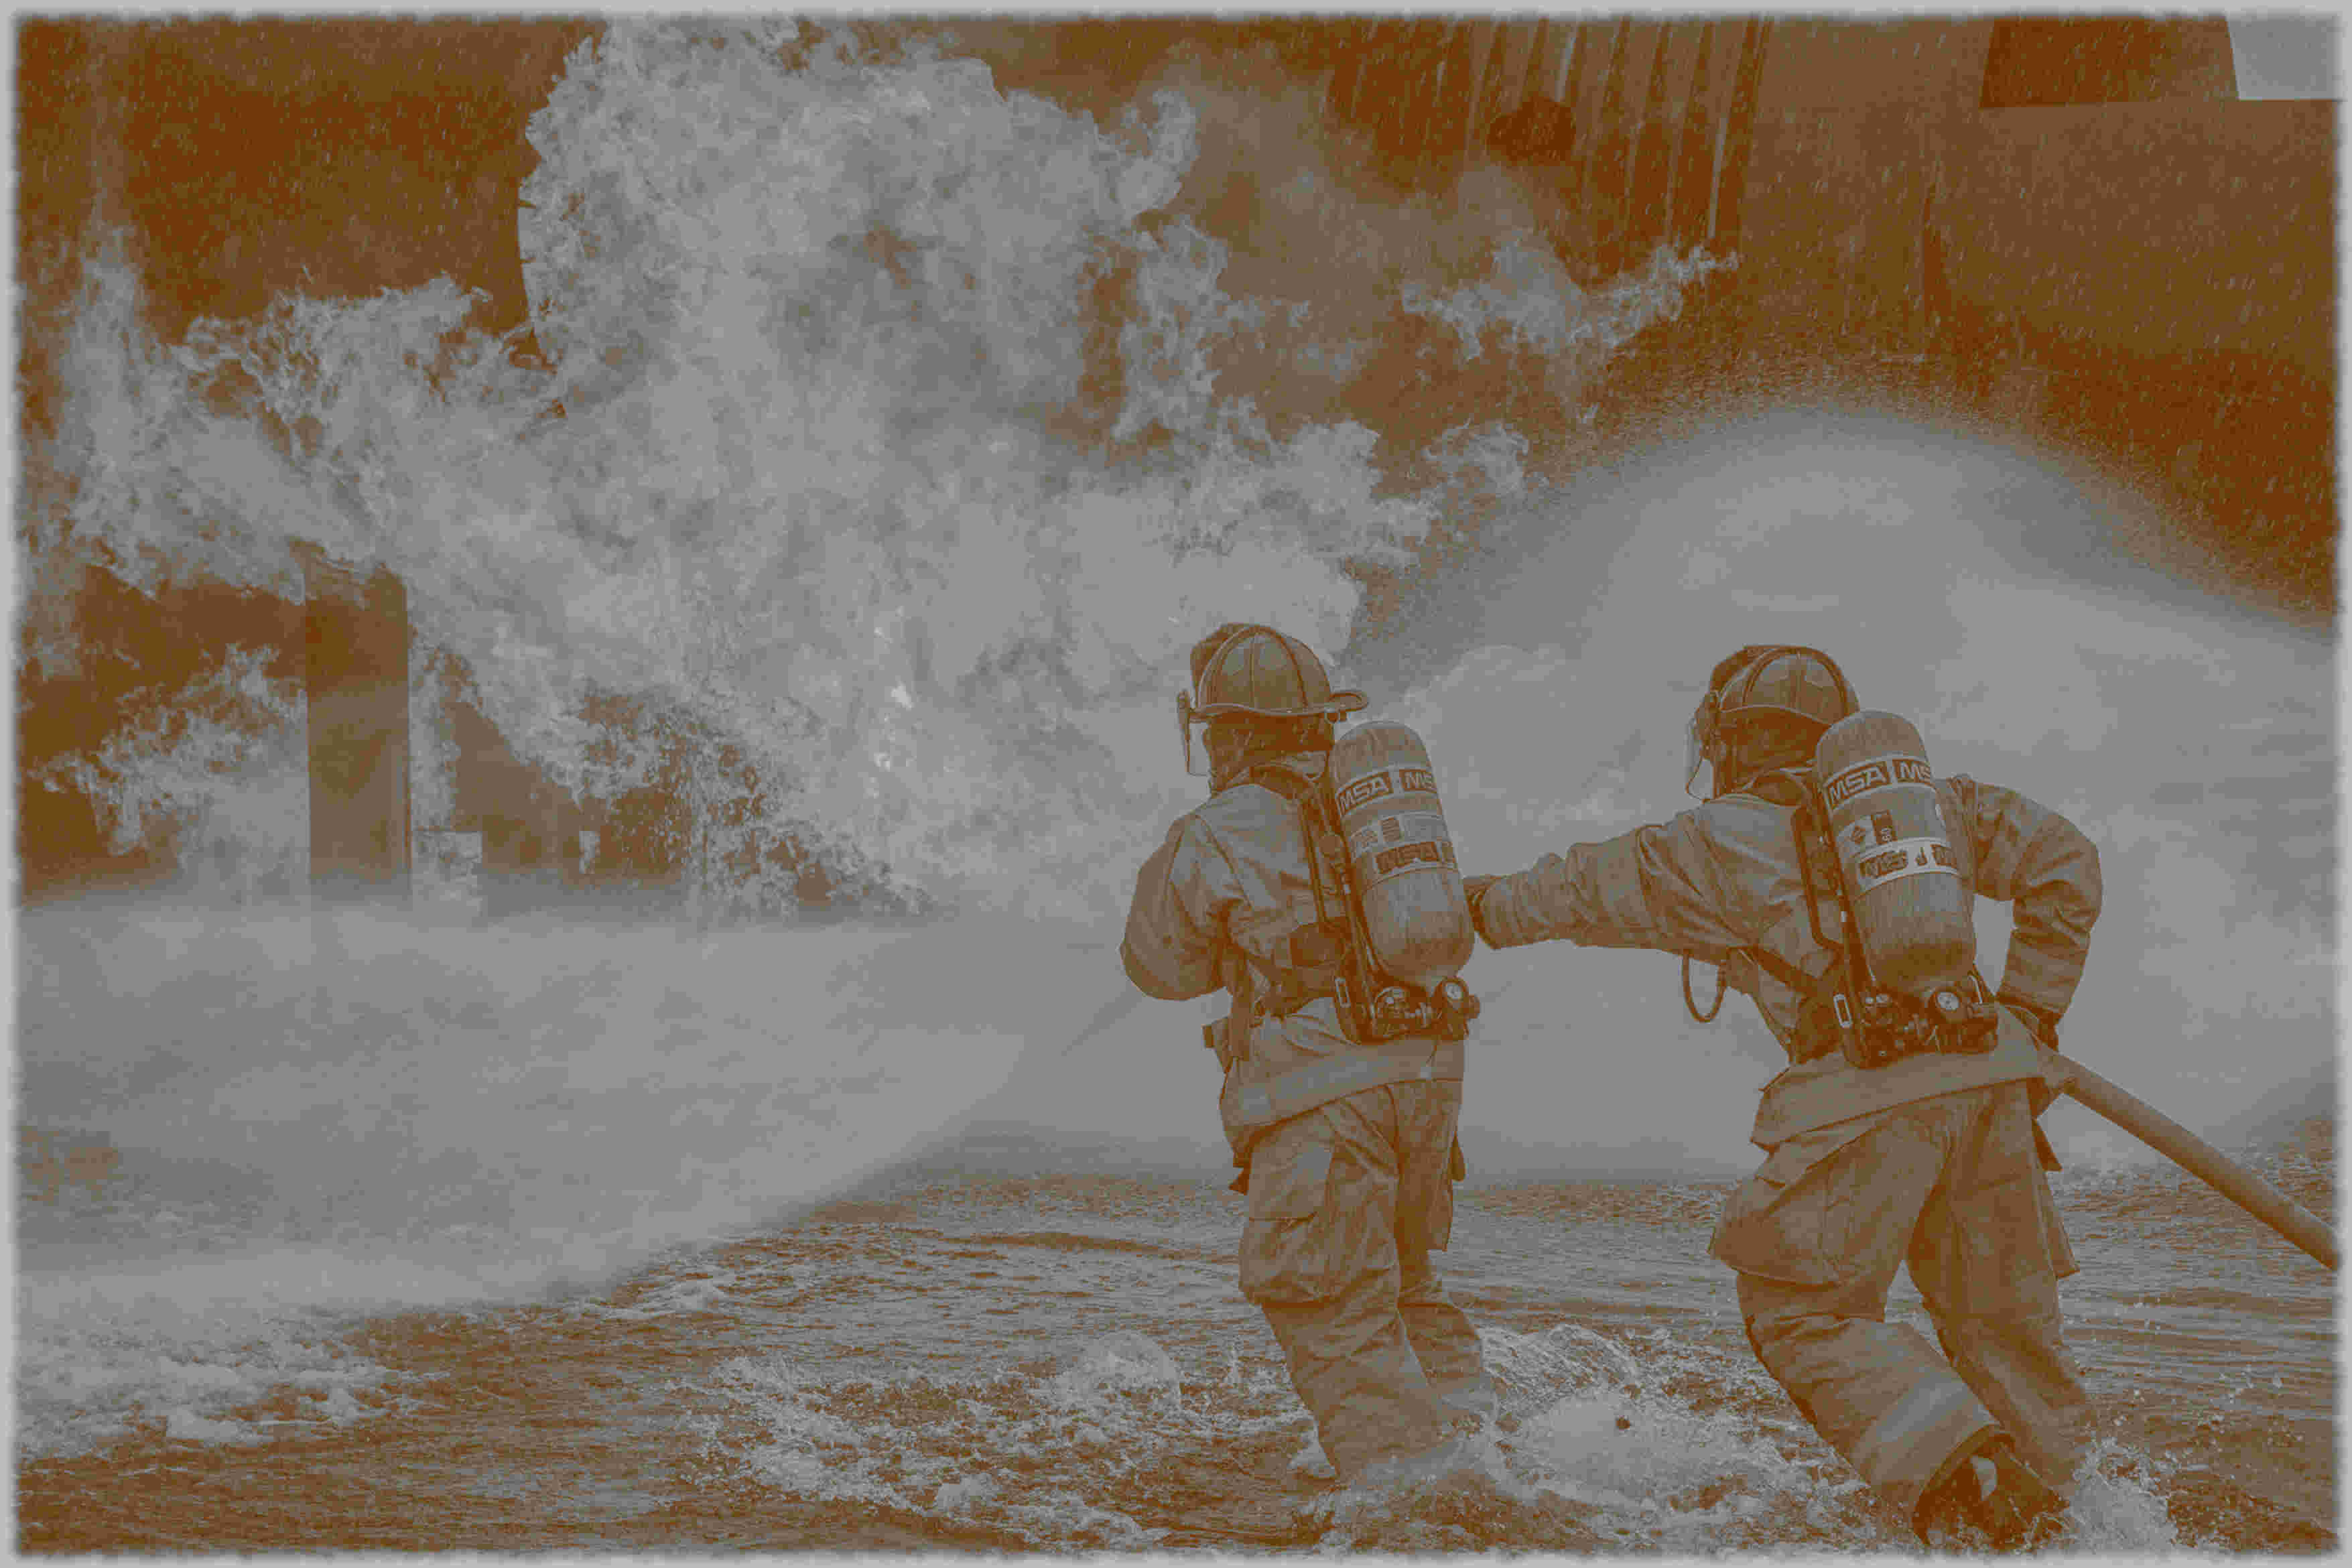
\includegraphics[height=150px]{Images/filters/old}
						\caption{Vieille photo}
				\end{figure}
		}

		\only<6>{
			\item[]
				\begin{figure}[H]
					\centering
						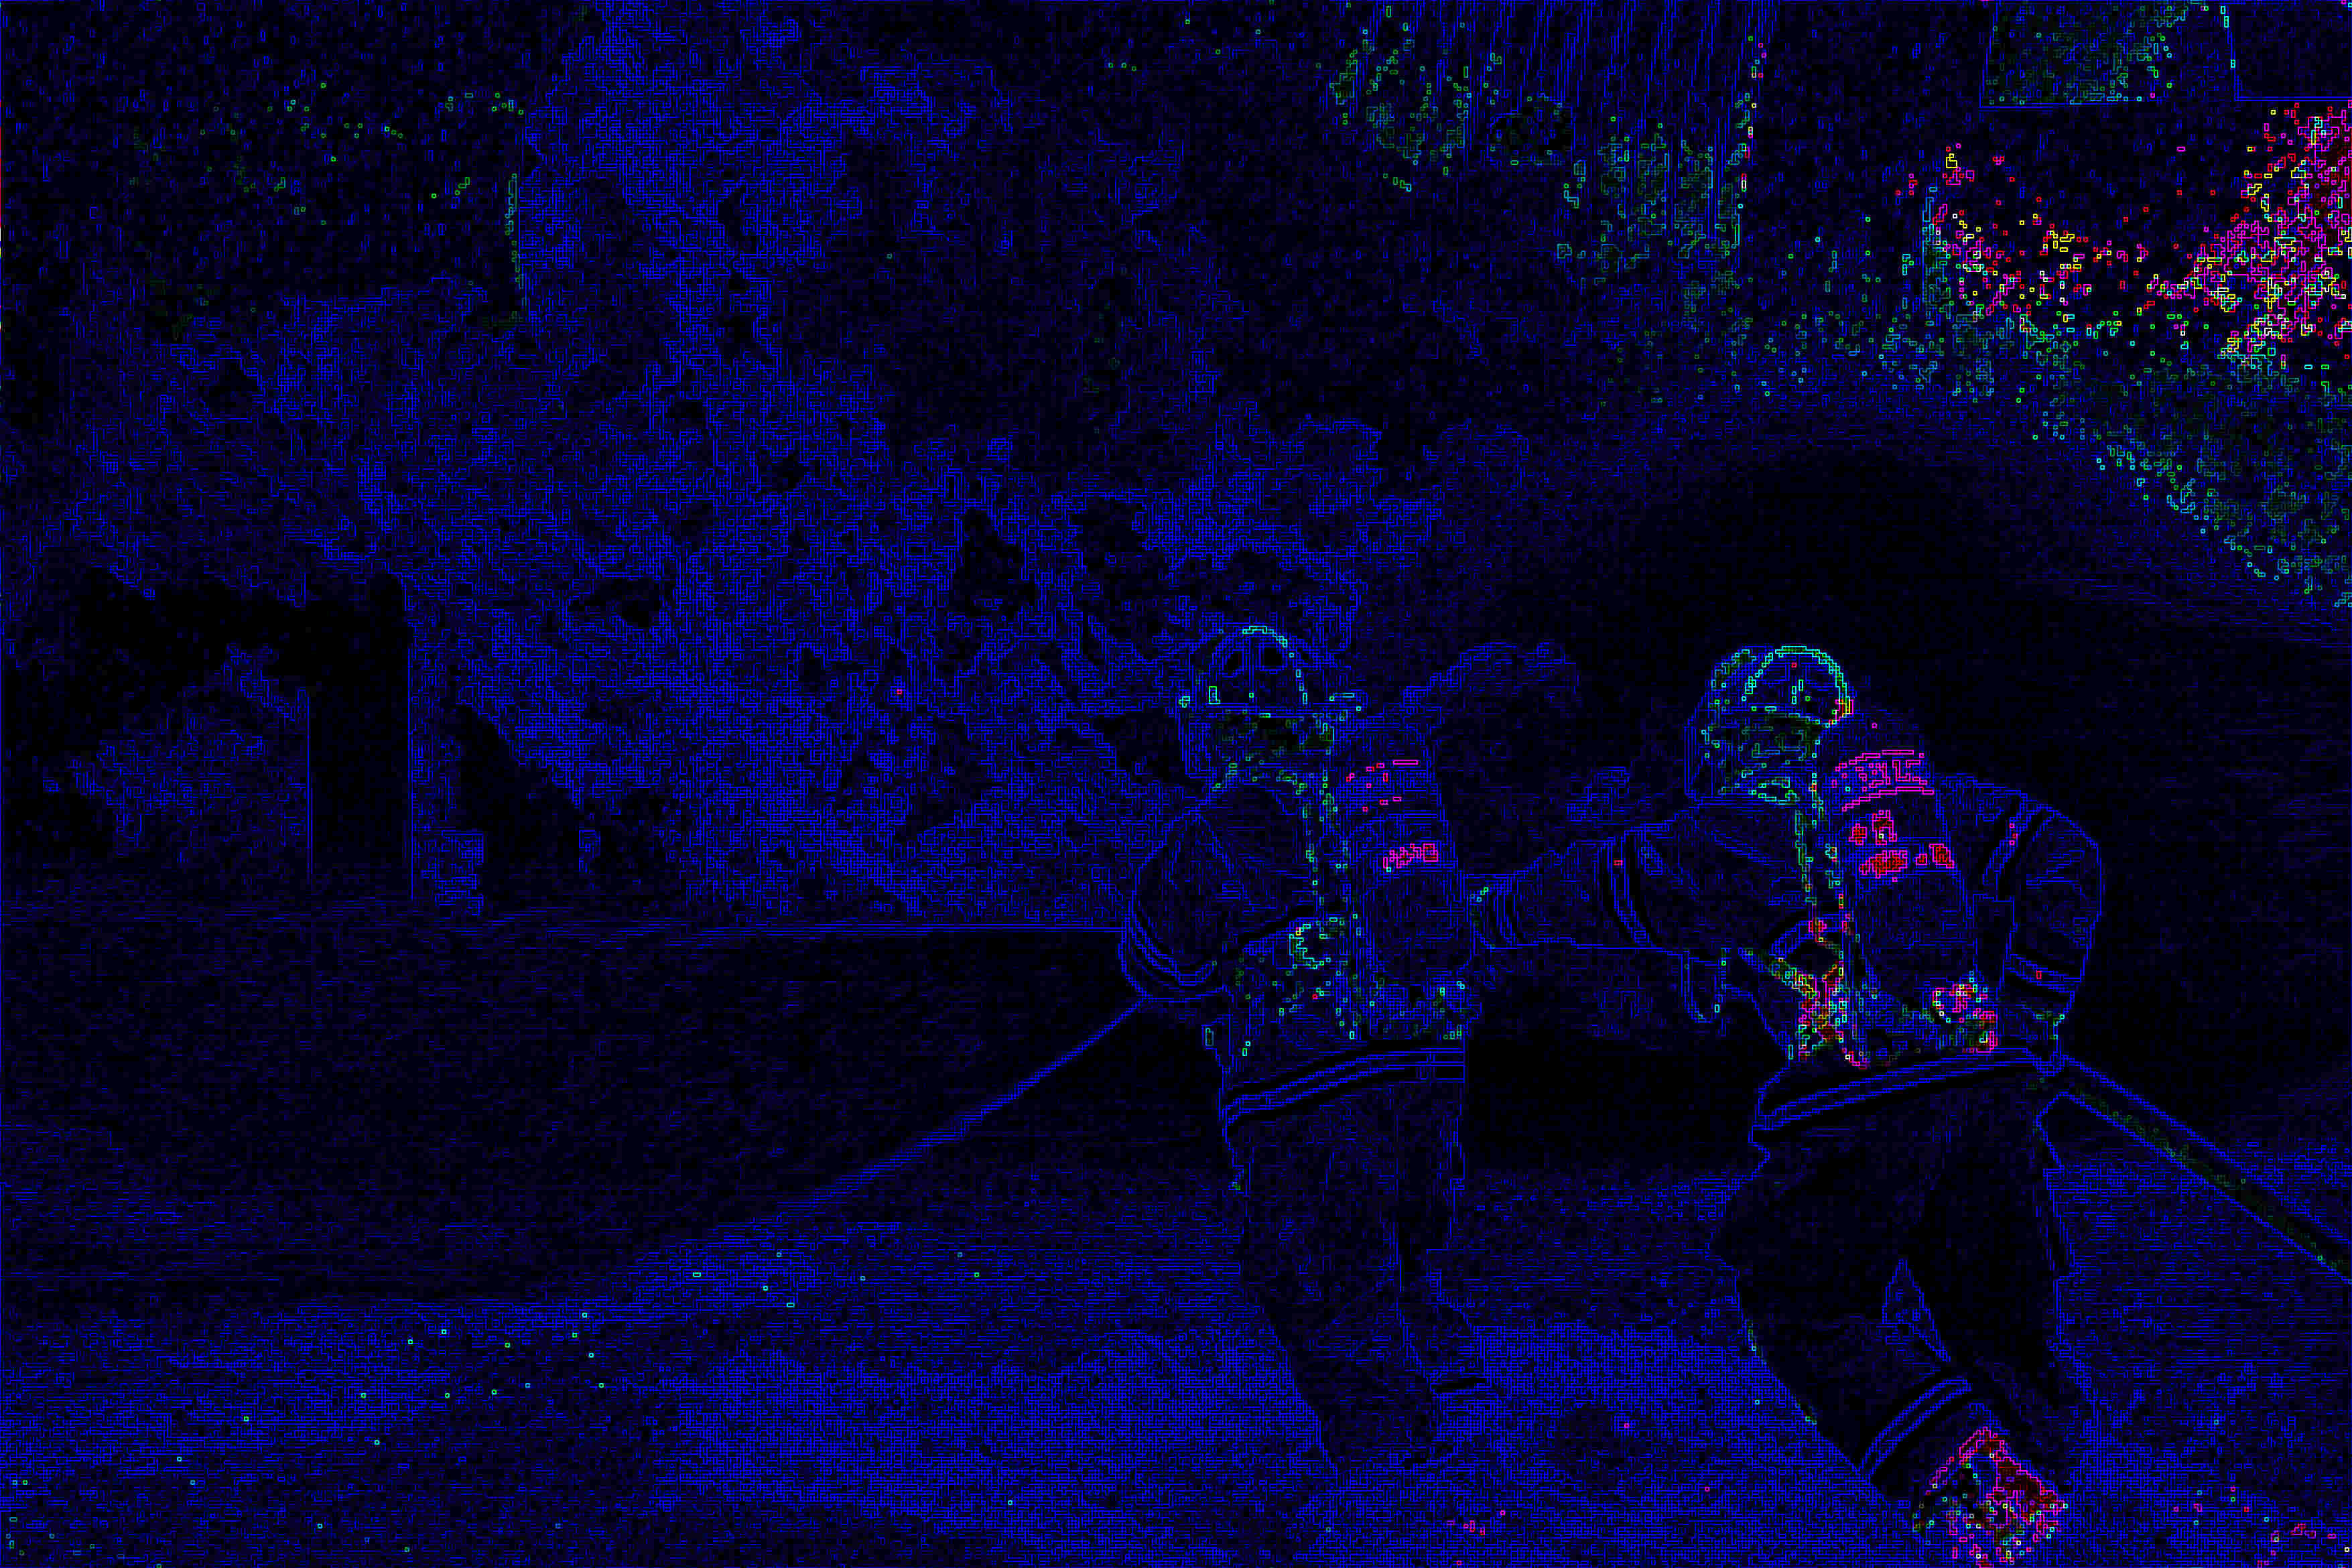
\includegraphics[height=150px]{Images/filters/predator}
						\caption{Prédateurs}
				\end{figure}
		}

		\only<7>{
			\item[]
				\begin{figure}[H]
					\centering
						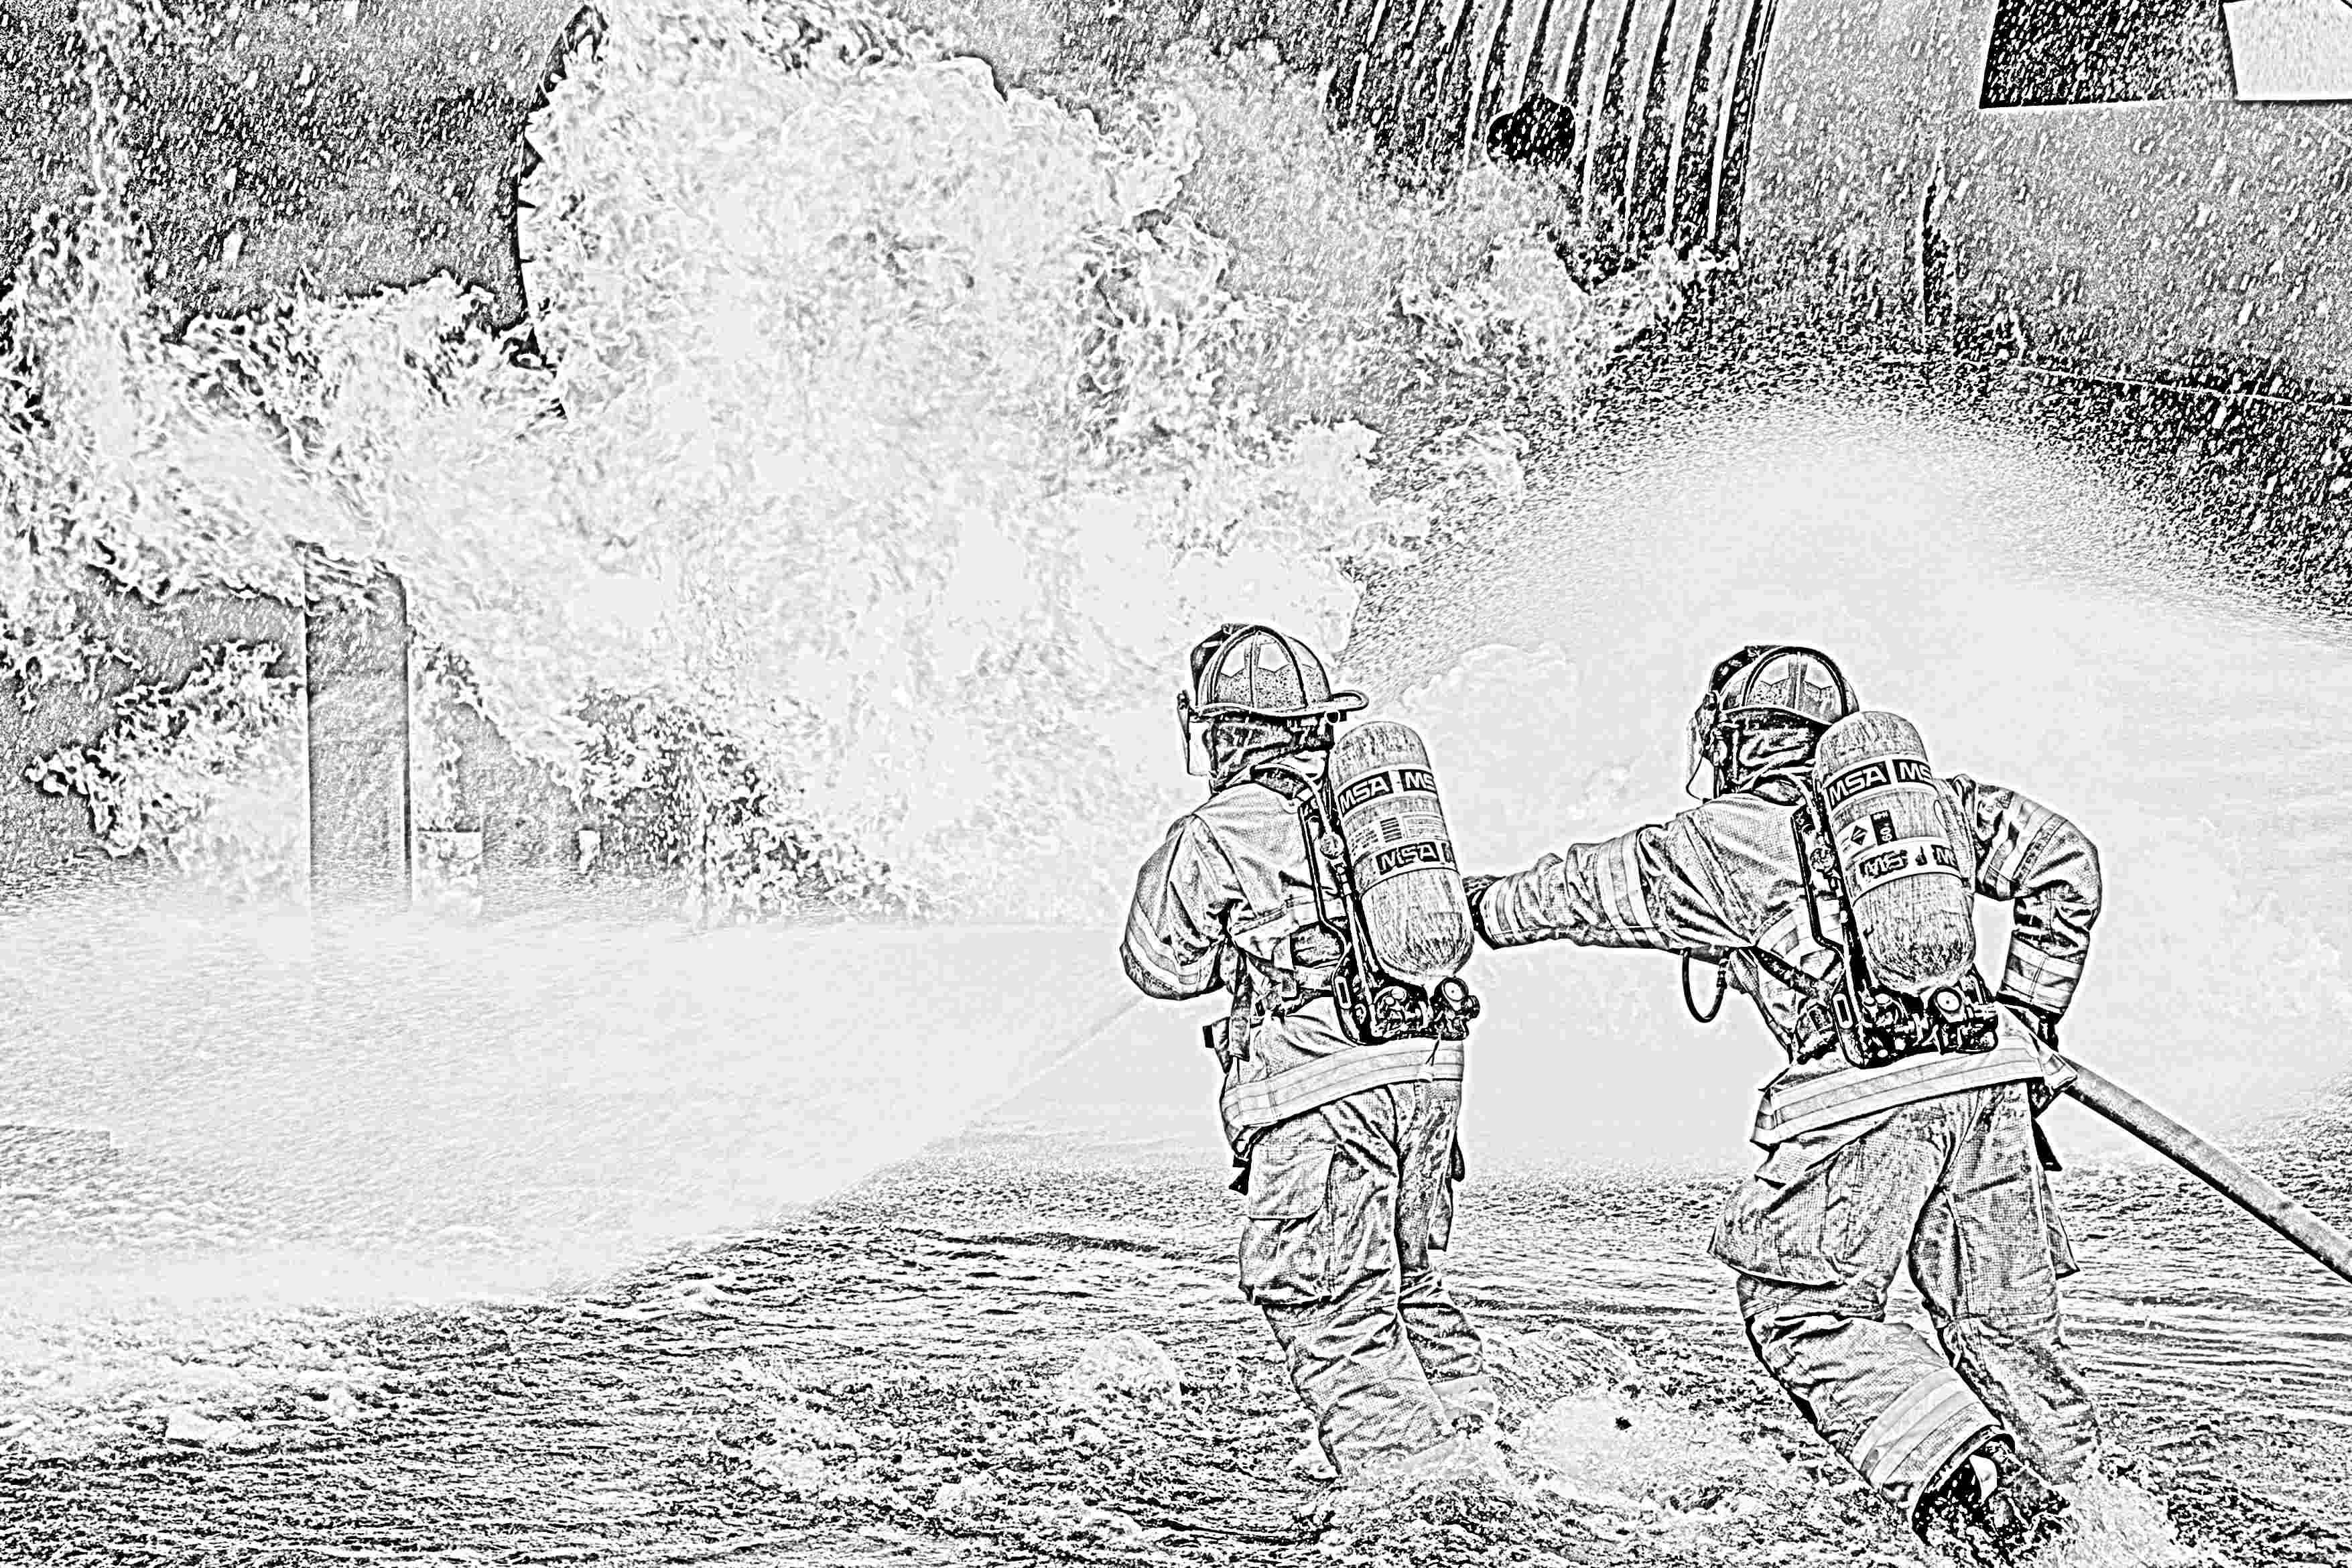
\includegraphics[height=150px]{Images/filters/photocopy}
						\caption{Photocopie}
				\end{figure}

		}

	\end{enumerate}
	\end{overprint}

\end{frame}

\begin{frame}{Filtres}
	Une liste des filtres de base (ainsi que des exemples) est disponible sur le lien suivant:

	\fbox{\footnotesize{\url{https://alvinalexander.com/design/gimp-catalog-filters-effects-examples-cheat-sheet}}}
%	\fbox{\url{http://goldnuggetwebs.com/gimp-filters/index.html}}

%% le premier site me parait meilleur mais la box dépasse du slide. Je verrai comment régler ça une fois  les slides plus avancés - L.

\end{frame}
